\chapter{Implementación y despliegue de la red.}

En este capítulo se expone el proceso de implementación de la red para cumplir los requisitos expuestos anteriormente. Empezamos generando un archivo de topología correcto a partir del esquema generado por MiniEdit para llegar a tener una simulación realista de la red, en la que los nodos no están configurados y tienen que obtener su propia configuración por parte de la red. Después implementamos la lógica de red para permitir la configuración dinámica de la misma sin necesidad de actuaciones manuales por parte de un operador. Finalmente exponemos como desplegar un entorno de pruebas para evaluar las prestaciones de la red.

En resumen, los pasos a seguir para implementar la red son:

\begin{itemize}
    \item Generar el archivo de topología final
    \item Preparar el servidor DHCP
    \item Activar el protocolo STP para evitar bucles.
    \item Activar el descubrimiento de topología de la red para distinguir enlaces trunk y de acceso
    \item Implementar el reenvío de paquetes condicionado por VLANs.
\end{itemize}


%\todo{quizás se podría llamar: diseño y despliegue de la rd? No suena bien desarrollo, en este contexto. DONE. ¿Aquí capturas de código entero o solo las partes relevantes?}
\section{Despliegue de la red en Mininet}

El archivo generado por MiniEdit contiene una serie de parámetros de configuración que no deseamos tener. Estos son, principalmente la asignación de direcciones IP a los nodos de la red. Como nuestro objetivo es que la red sea autoconfigurable tenemos que eliminar dichos parámetros. Además, ya que la identificación de nodos está basada en su dirección MAC tenemos que ajustar dichas direcciones a unos valores conocidos de antemano. Esto es así ya que si no damos ningún valor a las direcciones MAC estas se generan de forma aleatoria al arrancar Mininet, lo que hace que solo tengamos nodos en una VLAN (la VLAN por defecto).

Por esto hacemos los siguientes cambios a la configuración de los nodos:

\begin{lstlisting}[language=python, label=lst:miniedit-host, caption={Determinación de las direcciones MAC en los hosts Mininet}]
# h1 = net.addHost('h1', cls=Host, ip='10.0.0.2/24')
# h2 = net.addHost('h2', cls=Host, ip='10.0.0.3/24')
# ...

h1 = net.addHost('h1', cls=Host, ip=None, mac='00:00:00:00:00:01')
h2 = net.addHost('h2', cls=Host, ip=None, mac='00:00:00:00:00:02')
# ...

\end{lstlisting}

Así mismo tenemos que activar el soporte de la versión 1.3 del protocolo OpenFlow, ya que por defecto solo está activa la versión 1.0.

\begin{lstlisting}[language=python, label=lst:miniedit-switch, caption={Activación del protocolo OF1.3 en switch Mininet}]
s1 = net.addSwitch('s1', cls=OVSKernelSwitch, protocols="OpenFlow13")
\end{lstlisting}

Una vez arrancamos la red por primera vez y hacemos una captura de tráfico inicial comprobamos que está siendo inundada por paquetes de tipo ICMPv6 relacionados con el protocolo SLAAC de autoconfiguración de IPv6 \cite{rfc4862}. Como no estamos interesados en la configuración de IPv6 en nuestra red vamos a desactivar el protocolo en todos los nodos de la red. Para ello añadimos las siguientes líneas a nuestro script.

\begin{lstlisting}[language=python, label=lst:miniedit-ipv6, caption={Desactivación de IPv6 en nodos Mininet (Linux)}]
    info( '*** Desactivar IPv6\n')
    for h in net.hosts:
        h.cmd("sysctl -w net.ipv6.conf.all.disable_ipv6=1")
        h.cmd("sysctl -w net.ipv6.conf.default.disable_ipv6=1")
        h.cmd("sysctl -w net.ipv6.conf.lo.disable_ipv6=1")
\end{lstlisting}

Además tenemos que activar el protocolo DHCP, tanto en los clientes como en el servidor para poder proporcionar configuración automática de los equipos. Para esto añadimos al final del fichero de topología las siguientes líneas:

\begin{lstlisting}[language=python, label=lst:miniedit-dhcp, caption={Activación del servidor y clientes DHCP al arranque de la red.}]
info( '*** Iniciando el servidor DHCP \n')
    router.cmd("systemctl stop isc-dhcp-server")
    router.cmd("rm /var/lib/dhcp/dhcpd.leases")
    router.cmd("rm /var/lib/dhcp/dhcpd.leases~")
    router.cmd("touch /var/lib/dhcp/dhcpd.leases")
    router.cmd("dhcpd -4 -f --no-pid &")
    
    info( '*** Habilitando DHCP en los hosts\n')
    for h in net.hosts:
    	if h != router:
        	h.cmd("dhclient &")
\end{lstlisting}

Con estos cambios introducidos en el fichero de topología ya tenemos un conjunto de redes interconectados entre sí que simula el escenario propuesto por este trabajo y sobre el que ya podemos empezar a hacer pruebas del controlador SDN.


\section{Infraestructura de Ryu}

Ryu es un framework SDN escrito en Python basado en una estructura de aplicaciones independientes que se comunican entre sí mediante un bucle de eventos. Por esto es capaz de encadenar varias funcionalidades en un único controlador. Nuestra misión es escribir una aplicación Ryu que gestione diversos eventos relacionados con la red, siendo el principal evento a implementar el de la lógica de reenvío de paquetes. El controlador Ryu está encargado de determinar hacia donde se reenvían los paquetes que llegan a los distintos switches de la red y, si es necesario, de instalar las rutas en la tabla de rutas del switch para evitar que los paquetes sean enviados al controlador. Podemos ver un ejemplo básico de lógica de reenvío en la figura \ref{fig:primerpaquete}

\begin{figure}[!h]
    \centering
    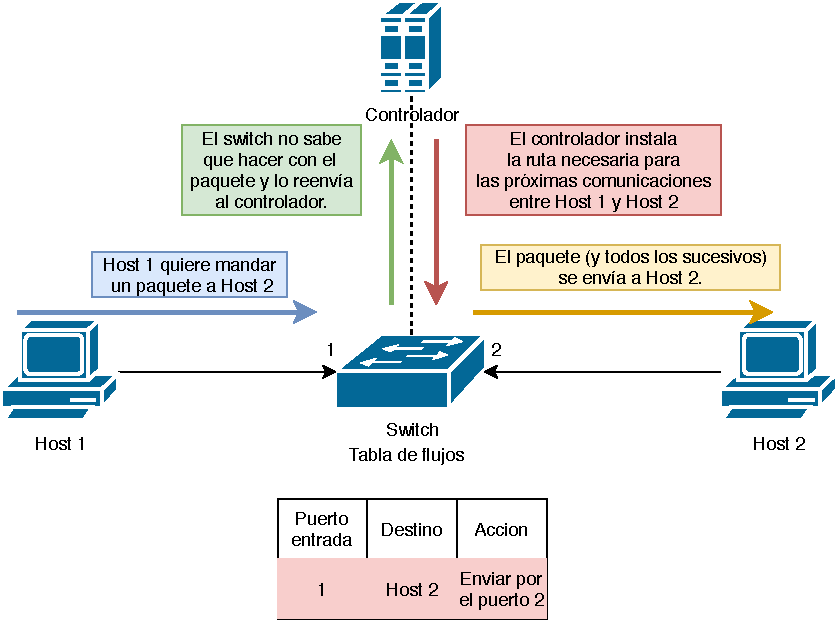
\includegraphics[width=\textwidth]{imagenes/figuras/primerpaquete.pdf}
    \caption{Ejemplo de instalación de ruta en la tabla de flujos de un switch OpenFlow}
    \label{fig:primerpaquete}
\end{figure}

En el flujo de control del controlador trabajamos únicamente respondiendo a eventos o mensajes de cualquiera de los switches o aplicación Ryu de una forma análoga a como lo hace un servidor web respondiendo peticiones de los usuarios. Para lograr una persistencia de datos y poder tomar decisiones sobre la red necesitamos persistencia de datos entre eventos en el controlador. Esto es fácilmente alcanzable mediante el uso de clases y objetos Python. Partimos de la base de que una aplicación Ryu es una clase en la que podemos guardar, por ejemplo, una descripción de la red o la tabla de direcciones MAC que conocemos.

Ahora vamos a describir las funcionalidades que hemos implementado en nuestro controlador Ryu: Switching, VLANs dinámicas, descubrimiento de topología y protocolo STP.

\subsection{Aplicación switch}

La base de todo switch es reenviar paquetes que entran al switch al nodo adecuado, evitando en la medida de lo posible enviar paquetes a nodos que no son el receptor. Con los switches tradicionales tenemos un hardware encargado de analizar los paquetes y reenviarlos al puerto adecuado de forma automática. Cuando estamos trabajando con switches SDN toda la funcionalidad tiene que ser implementada en el controlador. Esto tiene tanto ventajas (podemos configurar el reenvío como queramos) como desventajas (si nos olvidamos de alguna funcionalidad esta no estará disponible de forma automática).

Como punto de partida para nuestra aplicación hacemos una lectura de la aplicación integrada en Ryu llamada simple\_switch\_13.py. En esta aplicación se indica como programar un controlador SDN para implementar la funcionalidad básica de un switch tradicional (reenvío de paquetes con aprendizaje de direcciones MAC). A partir de este esquema podemos empezar a trabajar en nuestro propio controlador.

Una de las partes más relevantes es la primera regla que se añade a cada switch en cuanto se comunica por primera vez con el controlador. Esta regla indica que cualquier paquete que no cumpla ninguna de las reglas instaladas deberá ser enviado al controlador para decidir como procesarlo y, si es necesario, instalar una regla que coincida con futuros paquetes similares.

La creación de esta regla se hace respondiendo al evento \lstinline{ofp_event.EventOFPSwitchFeatures} generado al conectar un switch al controlador (bien porque se levanta el enlace o porque se reinician bien el switch, bien el controlador). La regla se instala de la siguiente manera.

\begin{lstlisting}[language=Python, label=lst:ryu-to-controller, caption={Instalación de la regla por defecto en un switch.}]
@set_ev_cls(ofp_event.EventOFPSwitchFeatures, CONFIG_DISPATCHER)
def switch_features_handler(self, ev):
    datapath = ev.msg.datapath #Objeto que representa al switch
    ofproto = datapath.ofproto #Protocolo openflow del switch
    parser = datapath.ofproto_parser
    dpid = datapath.id #Id del switch

    match = parser.OFPMatch() #No hay condiciones para cumplir esta regla
    #La accion de los paquetes que cumplan esta regla es enviarse al
    #controlador
    actions = [parser.OFPActionOutput(ofproto.OFPP_CONTROLLER,
                                      ofproto.OFPCML_NO_BUFFER)]
    #Anadir la regla al switch
    self.add_flow(datapath, 0, match, actions)
\end{lstlisting}



\subsection{VLAN dinámicas}

A partir de lo observado en el simple\_switch\_13 podemos empezar a trabajar en nuestro propio controlador. 

Podemos ver el diagrama de la funcionalidad que queremos implementar en la figura \ref{fig:decisiones-vlan1}. En nuestra red vamos a tener una topología cambiante y no vamos a saber en ningún momento en qué puerto específico se conecta cada nodo. Por esto vamos a basar nuestras decisiones de reenvío en la dirección MAC de los nodos origen y destino de cada paquete. Además tenemos que soportar nodos que pertenecen a más de una VLAN como el servidor/router de la red. En una red tradicional sabemos a que puerto pertenece cada VLAN porque lo hemos asignado previamente. En nuestra red tendremos que hacer estas averiguaciones en tiempo de ejecución para lograr una red completamente autoconfigurable.

\begin{figure}[!h]
    \centering
    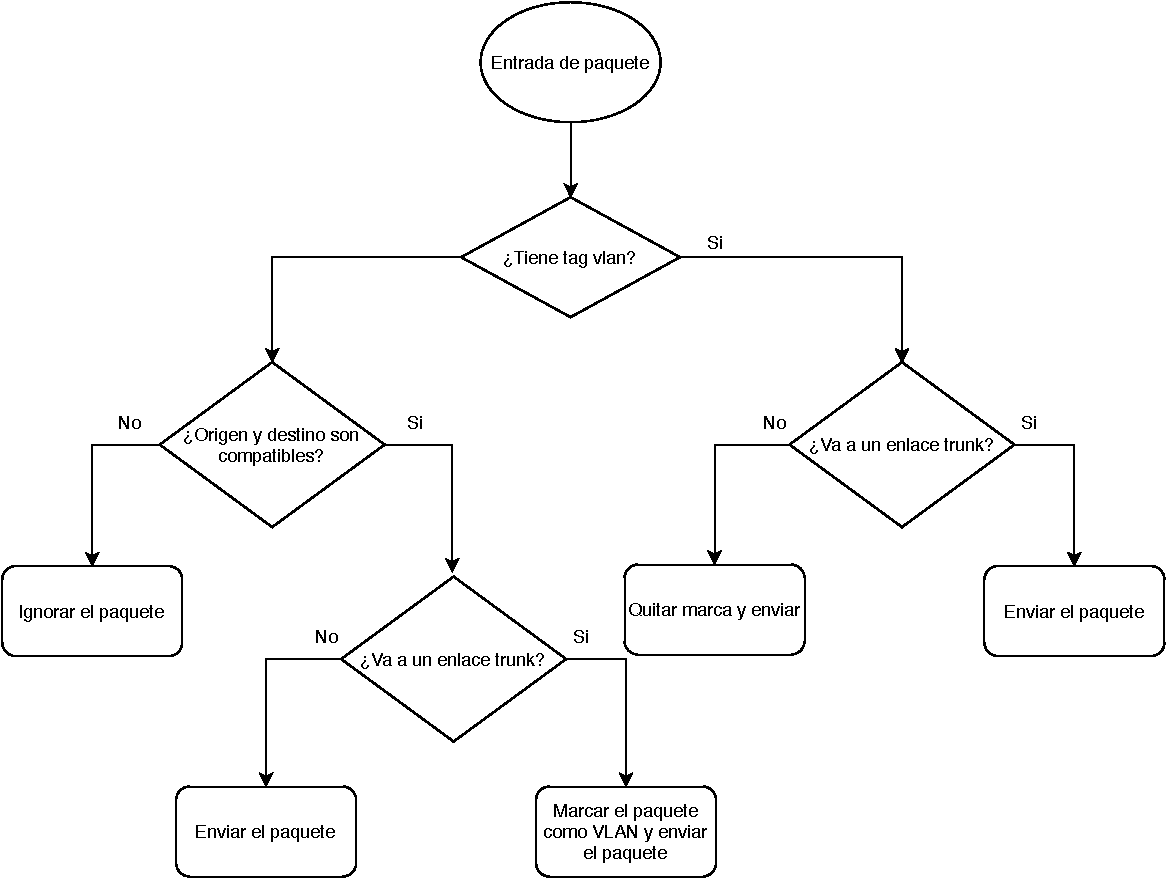
\includegraphics[width=\textwidth]{imagenes/figuras/decisiones_vlan.pdf}
    \caption{Diagrama de flujo del reenvío con VLAN}
    \label{fig:decisiones-vlan1}
\end{figure}

Empezamos creando una clase que nos permita saber a que VLAN pertenece cada nodo en función de su dirección MAC. La clase creada es la siguiente:

\begin{lstlisting}[language=Python, label=lst:vlan-assigner, caption={Clase encargada de determinar a que VLAN pertenece un nodo}]
class VlanAssigner():
    def __init__(self):
        self.vlans = [10,20,30] #Vlans disponibles
        self.default_vlan = 10 # Vlan por defecto
        self.macs_wildcards = {
            10 : [ #Vlan por defecto, trafico general
                'c2:c3:ae:8e:bf:25' #Mac del servidor
            ],
            20 : [ #Vlan de seguridad
                '01:ab:*',
                'c2:c3:ae:8e:bf:25' #Mac del servidor
            ],
            30 : [ #Vlan de telefonia
                '02:cd:*',
                'c2:c3:ae:8e:bf:25', #Mac del servidor
                '48:*'
            ]
        }

    def match_vlan(self,mac):
        encontrado = False
        resultado = []

        for k,v in self.macs_wildcards.items():
            for exp in v:
                r = re.compile(exp)
                if r.match(mac):
                    encontrado = True
                    resultado.append(k)
        if not encontrado:
            resultado.append(self.default_vlan)
        
        resultado.sort()
        return resultado
\end{lstlisting}

Ahora podemos empezar a implementar la lógica de reenvío de paquetes. Un problema con el que nos encontramos es que los paquetes broadcast (sean ARP o DHCP) no pueden enviarse debido a que la red no sabe a qué nodo van dirigidos (dirección destino ff:ff:ff:ff:ff:ff) por lo que los nodos no pueden establecer conexiones entre sí (no pueden resolver su mac a partir de su ip).

Por el problema descrito anteriormente tenemos que modificar la lógica de reenvío de paquetes de la siguiente manera:

\begin{figure}[!h]
    \centering
    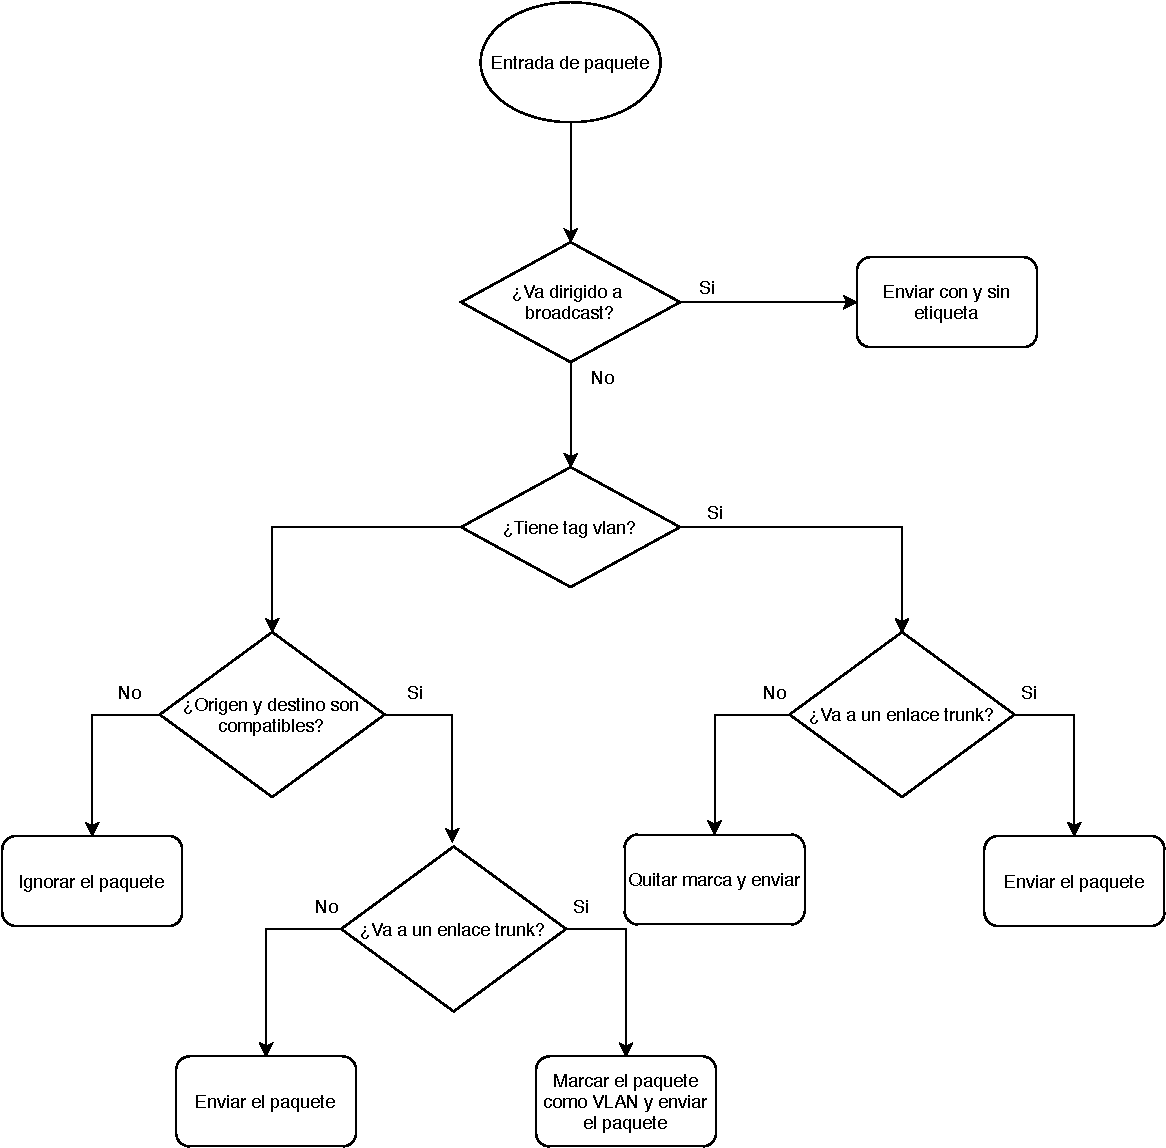
\includegraphics[width=\textwidth]{imagenes/figuras/decisiones_vlan2.pdf}
    \caption{Diagrama de flujo del reenvío con VLAN teniendo en cuenta direcciones broadcast}
    \label{fig:decisiones-vlan2}
\end{figure}

Como podemos ver en la figura \ref{fig:decisiones-vlan2} los paquetes broadcast se envían duplican: unos llevan tag VLAN y otros no. Aunque esto puede parecer un problema no lo es ya que las tarjetas de red ignoran los paquetes encapsulados en una VLAN si esta no está configurada explícitamente.

Una vez tenemos resuelto el problema de los paquetes broadcast podemos terminar de implementar la lógica de reenvío.

Si nos llega un paquete procedente de una VLAN puede venir de un host multiVLAN o de otro switch (recordemos que las decisiones de reenvío son individuales para cada switch). Tenemos que determinar primero si los host origen y destino pertenecen a la misma VLAN. Para ello hacemos uso de la siguiente función:

\begin{lstlisting}[language=Python, label=lst:vlan-compatible, caption={Función que determina si dos nodos pertenencen a la misma VlAN}]
def vlan_compatibles(self,src,dst):
    vlan_src = self.v.match_vlan(src)
    vlan_dst = self.v.match_vlan(dst)
    for v in vlan_src:
        if v in vlan_dst: return v
    return False
\end{lstlisting}

Si ambos nodos pueden comunicarse entre ellos enviamos el paquete al puerto donde sabemos que se encuentra el nodo (o el switch que se comunica con el nodo). Tenemos que discernir entre si estamos enviando a un puerto trunk o a un puerto de acceso. Como esto no lo sabemos a priori hacemos uso de la api de descubrimiento de topología de ryu. Si es un puerto trunk enviamos el paquete tal como nos ha entrado. Si es un puerto de acceso quitamos las marcas de VLAN mediante la acción \lstinline{OFPActionPopVlan()} de OpenFlow 1.3 y enviamos el paquete. Si no sabemos a que puerto tenemos que enviar el paquete (porque no conocemos todavía en nuestro switch al destinatario) enviamos el paquete por todos los puertos disponibles. Si conocemos al destinatario y el paquete se puede enviar instalamos una nueva regla de reenvío en el switch de forma que el próximo paquete dirigido a dicho nodo destino por la misma VLAN sea reenviado de forma transparente por el switch sin tener que volver a ejecutar este algoritmo en el controlador.

En caso que nos llegue un paquete sin marca de VLAN seguimos un proceso similar al anteriormente descrito pero añadiendo mediante la instrucción \lstinline{OFPActionPushVlan()} de OpenFlow su correspondiente marca.

Todo el código puede ser consultado en el repositorio del trabajo en el archivo controlador\_vlan.py.

\subsection{Descubrimiento de topología}

Para poder determinar si un puerto es trunk o no tenemos que saber donde está conectado: si está conectado a un nodo final es un puerto de acceso, si lo está a otro switch es un puerto trunk (entre switches todos los paquetes viajan taggeados). Para eso vamos a hacer uso de la api de descubrimiento de topología de Ryu que, mediante intercambio de paquetes de tipo \acrshort{lldp} \footnote{Link Layer Discovery Protocol, Protocolo de intercambio de información entre vecinos a nivel 2 (enlace)}, nos permite conocer la topología de nuestra red activa. De esta forma aprovechamos esta función para crear la siguiente función que determina si un puerto es trunk o de acceso:

\begin{lstlisting}[language=Python, label=lst:is-trunk, caption={Función que determina si un puerto es de tipo trunk}]
def is_trunk(self, dpid, port_no):
    links_list = get_link(self, dpid)
    links=[link.src.port_no for link in links_list]
    return (port_no in links)
\end{lstlisting}

En el código anterior la función \lstinline{get_link} nos devuelve los enlaces entre switches del switch con identificador \lstinline{dpid}.

De igual manera podemos conocer si un host pertenece a múltiples VLANs y por tanto su puerto es de tipo trunk contando a cuantas VLAN pertenece. Si es a más de una es un nodo miembro de varias VLAN y deberá recibir los paquetes marcados.


\subsection{Aplicación STP}

En la red que estamos implementando tenemos varios enlaces redundantes para asegurar la disponibilidad del sistema. Esta decisión de diseño trae un problema aparejado: tenemos que eliminar los bucles de la red para evitar el fenómeno conocido como tormenta de broadcast (véase figura  \cite{Spanning33:online}. Ryu tiene una librería integrada que implementa el protocolo STP y bloquea los puertos que hacen que haya bucles en la red.

\begin{figure}[!h]
    \centering
    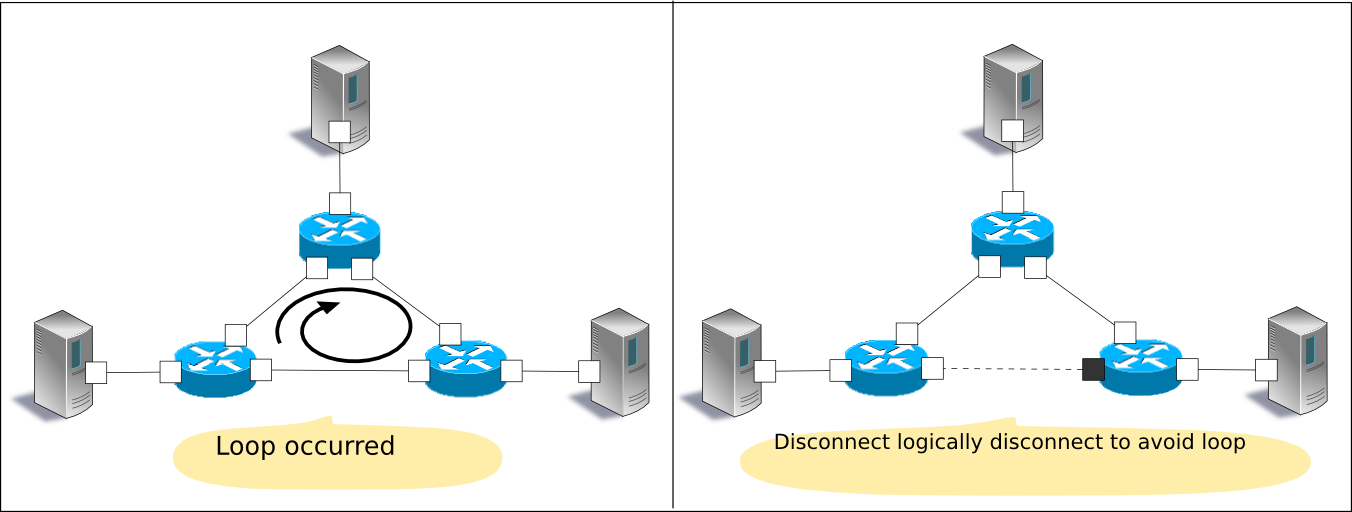
\includegraphics[width=\textwidth]{imagenes/figuras/stp.png}
    \caption{Motivación para utilizar STP. Fuente: ryu-book \cite{Spanning54:online}}
    \label{fig:motivacion-stp}
\end{figure}

Para activar el protocolo STP lo habilitamos en los contextos de nuestra aplicación

\begin{lstlisting}[language=Python, label=lst:stp-enable, caption={Activación del protocolo STP}]
_CONTEXTS = {
    'stplib': stplib.Stp
}
def __init__(self, *args, **kwargs):
    super(VlanSwitch,self).__init__(*args,**kwargs)
    self.mac_to_port = {}
    self.v = VlanAssigner()
    # Integracion de STPLib
    self.stp = kwargs['stplib']
\end{lstlisting}

Una vez hemos añadido el código indicado en \ref{lst:stp-enable} nuestra red ya ejecuta el protocolo STP. Si cae algún enlace o se activa uno nuevo el protocolo se vuelve a ejecutar de forma automática, permitiendo que la red responda dinámicamente a posibles cambios en la topología.


\section{Servicios auxiliares en el servidor}

Para poder correr la red y hacer pruebas sobre ella nos hace falta un nodo que actúe de servidor. Su tarea principal es servir direcciones mediante DHCP aunque también podría funcionar como servidor de contenido o como puerta de enlace hacia otras redes.

Lo primero que necesitamos es instalar un par de paquetes (suponiendo una distribución Linux basada en Debian)

\begin{lstlisting}[language=bash, label=lst:install-dhcp, caption={Instalación de paquetes en el servidor de la red.}]
sudo apt install vlan isc-dhcp-server
sudo modprobe 8021Q
\end{lstlisting}

\subsection{Servidor DHCP}

Además tenemos que modificar el archivo de configuración que se encuentra en \lstinline{/etc/dhcp/dhcpd.conf} para incluir una configuración similar a esta.

\begin{lstlisting}[language=bash, label=lst:dhcp-conf, caption={Configuración del servidor DHCP para servir a múltiples VLANs}]
subnet 10.0.0.0 netmask 255.255.255.0 {
  range 10.0.0.10 10.0.0.250;
  option domain-name-servers 8.8.8.8;
  option subnet-mask 255.255.255.0;
  option routers 10.0.0.1;
  option broadcast-address 10.0.0.255;
  default-lease-time 600;
  max-lease-time 7200;
  INTERFACES="router-eth0.10";
}

subnet 10.0.1.0 netmask 255.255.255.0 {
  range 10.0.1.10 10.0.1.250;
  option domain-name-servers 8.8.8.8;
  option subnet-mask 255.255.255.0;
  option routers 10.0.1.1;
  option broadcast-address 10.0.1.255;
  default-lease-time 600;
  max-lease-time 7200;
  INTERFACES="router-eth0.20";
}

subnet 10.0.2.0 netmask 255.255.255.0 {
  range 10.0.2.10 10.0.2.250;
  option domain-name-servers 8.8.8.8;
  option subnet-mask 255.255.255.0;
  option routers 10.0.2.1;
  option broadcast-address 10.0.2.255;
  default-lease-time 600;
  max-lease-time 7200;
  INTERFACES="router-eth0.30";
}
\end{lstlisting}

Con la configuración mostrada en el listado \ref{lst:dhcp-conf} conseguimos que el servidor DHCP escuche y atienda peticiones por todas las VLANs.

\section{Despliegue}

Una vez tenemos todo implementado y el servidor preparado procedemos a ejecutar el controlador y la red. Los pasos a seguir son los siguientes:

\subsection{Instalación de Mininet y Ryu}

En un entorno Linux basado en Ubuntu con python3 instalado ejecutamos los siguientes comandos para instalar Mininet-wifi y Ryu.

\begin{lstlisting}[language=bash, label=lst:install, caption={Instalación de Mininet-wifi y Ryu}]
git clone https://github.com/intrig-unicamp/mininet-wifi
cd mininet-wifi
sudo util/install.sh -Wlnfv
sudo pip install ryu
\end{lstlisting}

\subsection{Simulación de la red y ejecución del controlador}

Ahora podemos arrancar nuestra red virtualizada para hacer pruebas. Para ello tenemos que abrir dos consolas distintas.

\begin{enumerate}
    \item En la primera consola ejecutamos para arrancar el controlador Ryu:

\lstinline{sudo ryu-manager controlador_vlan.py --observe-links}

    \item En la segunda consola ejecutamos el script de topología de Mininet:

\lstinline{sudo python topologia_oficina.py}
\end{enumerate}

Teniendo estas dos consolas activas ya tenemos nuestra red funcionando. Desde la consola donde hemos ejecutado mininet podemos acceder a terminales de cada uno de los nodos de la red, así como ejecutar wireshark para hacer capturas de paquetes en cualquiera de los enlaces de la red.

\begin{figure}[!h]
    \centering
    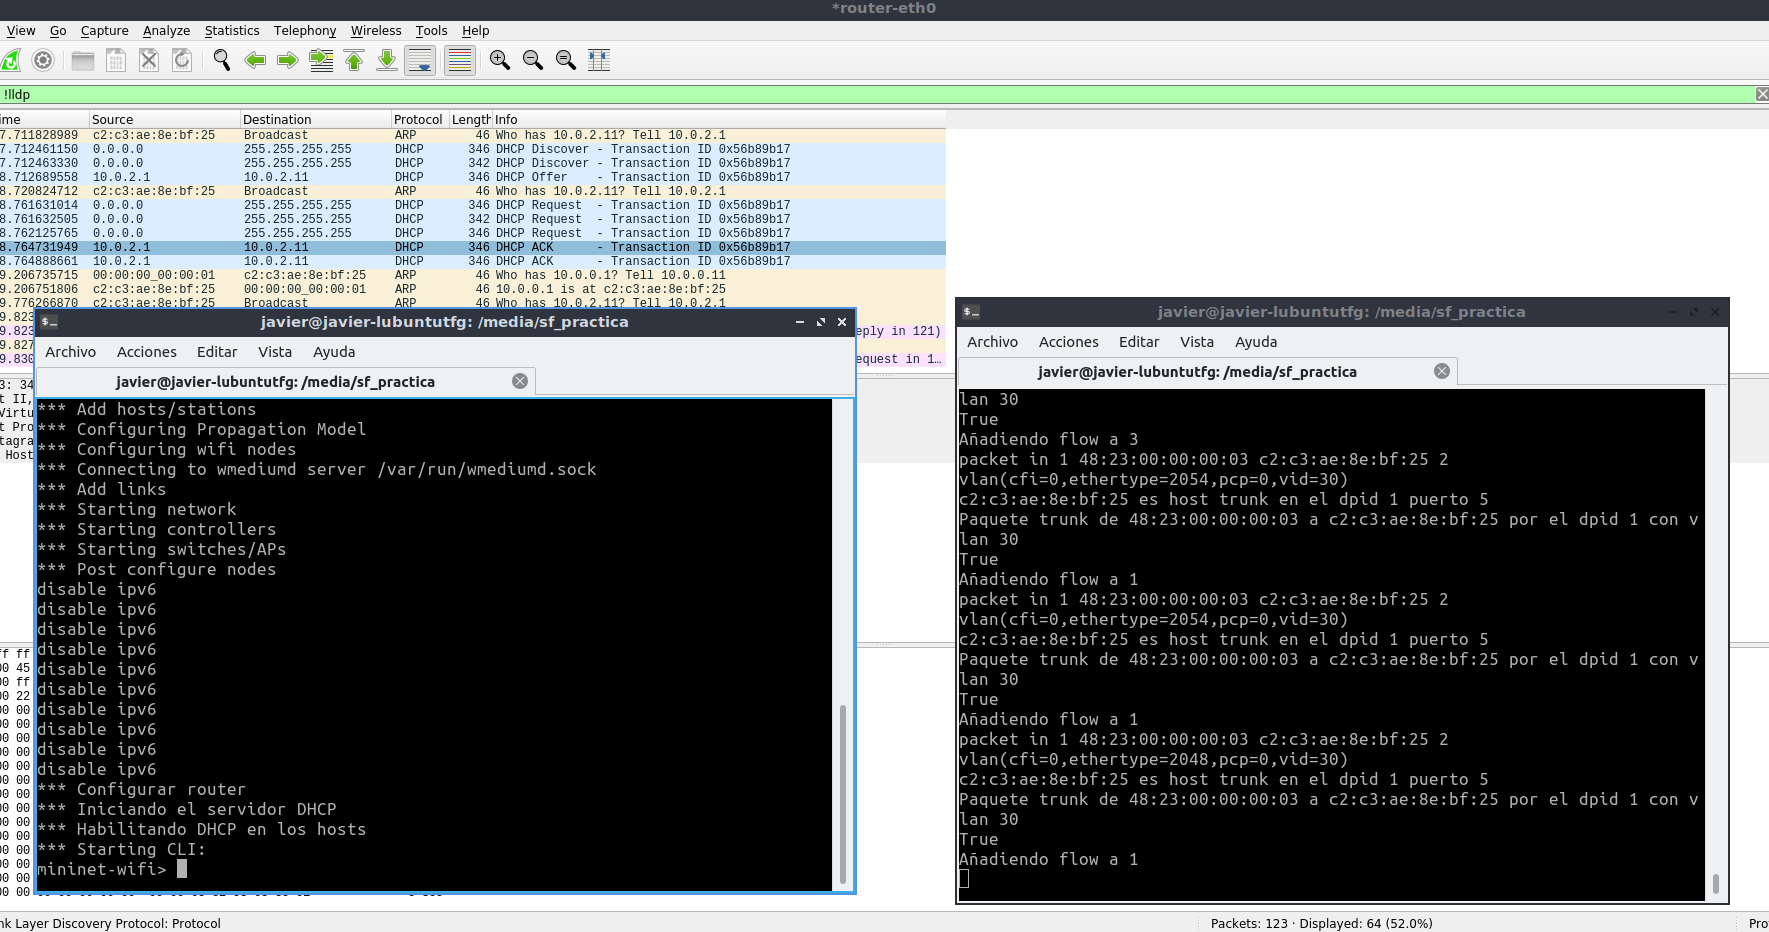
\includegraphics[width=\textwidth]{imagenes/figuras/red_funcionando.png}
    \caption{Red en funcionamiento con wireshark de fondo mostrando los paquetes que llegan al router.}
    \label{fig:red-funcionando}
\end{figure}
